\documentclass[11pt, a4paper]{article}


% Modules essentiels
\usepackage[french]{babel}
\usepackage[T1]{fontenc}
\usepackage[hmargin=2.5cm, vmargin=2.5cm]{geometry}
\usepackage[utf8]{inputenc}
\usepackage[skip=1em]{parskip}


% Modules supplémentaires
\usepackage[algoruled, lined, linesnumbered, longend, french, frenchkw]{algorithm2e}
\DontPrintSemicolon
\SetNlSty{tiny texttt}{}{}

\usepackage{amsfonts}
\usepackage{amsmath}
\usepackage{amssymb}

\usepackage{caption}

\usepackage{color}
\definecolor{mybordeaux}{rgb}{0.43, 0.03, 0.01}
\definecolor{mygray}{rgb}{0.95, 0.95, 0.95}
\definecolor{mygreen}{rgb}{0, 0.6, 0}
\definecolor{myred}{rgb}{0.6, 0, 0}
\definecolor{mypurple}{rgb}{0.73, 0.33, 0.83}

\usepackage{enumitem}
\setlist[itemize]{noitemsep, left=11pt}

\usepackage{graphicx}
\graphicspath{{../images/}{../../plots/}}

\usepackage{hyperref}
\addto\extrasfrench%
{%
	\def\algorithmautorefname{\textsc{Alg.}}
	\def\equationautorefname{\textsc{Éq.}}
	\def\figureautorefname{\textsc{Fig.}}
	\def\lstlistingautorefname{\textsc{List.}}
	\def\sectionautorefname{\textsc{Sec.}}
	\def\subsectionautorefname{\textsc{Sec.}}
	\def\subsubsectionautorefname{\textsc{Sec.}}
	\def\tableautorefname{\textsc{Tab.}}%
}

\usepackage{listings}
\lstset%
{%
	basicstyle=\ttfamily,
	backgroundcolor=\color{mygray},
	breaklines=true,
	captionpos=b,
	commentstyle=\color{mygreen},
	emph={},
	emphstyle=\color{mybordeaux},
	extendedchars=true,
	firstnumber=1,
	float,
	frame=single,
	keywordstyle=\color{myred},
	language=Python,
	literate= {À}{{\`A}}1 {à}{{\`a}}1 {é}{{\'e}}1 {è}{{\`e}}1,
	numbers=left,
	numberstyle=\tiny\color{black},
	showstringspaces=true,
	stepnumber=5,
	stringstyle=\color{mypurple},
	tabsize=3%
}

\usepackage[space-before-unit]{siunitx}

\usepackage{subcaption}

\usepackage{tabularx}


% Caractéristiques du document
\title{Traitement des données de sortie de LAMMPS}
\author{Heiarii Lou Chao}
%\date{}


\begin{document}
\maketitle
\tableofcontents

\clearpage
\section*{Introduction}

Nous nous penchons sur le traitement des données de sortie de LAMMPS, obtenues avec la commande \lstinline!dump!, pour calculer la fonction de distribution radiale (Radial Distribution Function, RDF) et le déplacement carré moyen (Mean Squared Displacement, MSD).

\section{Fichiers de sortie}

Les fichiers de sortie de LAMMPS obtenus avec la commande \lstinline!dump ... custom! ont un format spécifique, présenté au \autoref{lst:sortie_format}.

\begin{lstlisting}[caption={Format des données des fichiers de sortie}, label={lst:sortie_format}, floatplacement={hpbt}]
ITEM: TIMESTEP
...
ITEM: NUMBER OF ATOMS
...
ITEM: BOX BOUNDS pp pp pp
...
...
...
ITEM: ATOMS ...
...
\end{lstlisting}

Nous utilisons donc ceci comme repère pour lire les données : le fichier peut être décomposé en $N_{sorties} = N_{iterations} // T_{ecriture}$ (avec $T_{ecriture}$ la période itérative d'écriture de la commande \lstinline!dump!) portions de $\num{9} + N_{atomes}$ lignes.

Pour concevoir un programme flexible, nous partons du principe que le nombre d'itérations, la période itérative d'écriture et le nombre d'atomes ne sont pas connus à l'avance. Enfin pour faciliter le traitement des données, le fichier de sortie contiendra également les coordonnées "unwrapped" des atomes, c'est-à-dire sans l'application des conditions aux limites.

\section{Lecture des données}

Comme évoqué précédemment, nous faisons le choix de lire les données du fichier par portions. Aussi, pour le calcul de la RDF, il est essentiel de connaître les dimensions de la boîte de simulation.\\
Il est donc nécessaire de lire la nombre d'atomes et les dimensions de la boîte de simulation \emph{avant} de parcourir les données du fichier (\autoref{fig:lecture_prealable}).

\begin{figure}[hbpt]
	\centering
	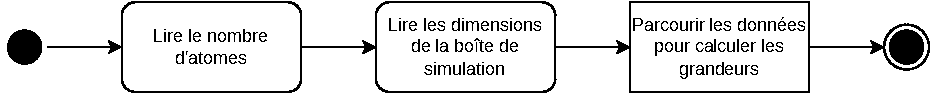
\includegraphics[width=\linewidth]{demarche-preliminaires.pdf}
	\caption{Lecture préalable des données}
	\label{fig:lecture_prealable}
\end{figure}

Une fois ceci fait, le fichier des données peut être parcouru pour le calcul des grandeurs (\autoref{fig:lecture_calcul}).

\begin{figure}[hptb]
	\centering
	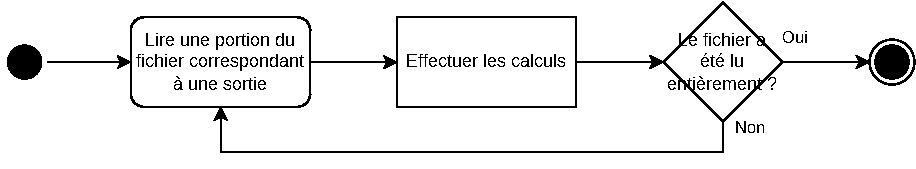
\includegraphics[width=\linewidth]{demarche-lecture.pdf}
	\caption{Lecture des données et calcul des grandeurs}
	\label{fig:lecture_calcul}
\end{figure}

\section{Fonction de distribution radiale}

Pour calculer la fonction de distribution radiale, nous nous référons à \emph{Computer Simulation of Liquids}, \textsc{M. P. Allen} et \textsc{D. J. Tildesley}, p. 69 et 272.

	\subsection{Rappels théoriques}

Dans cet ouvrage, l'expression de la fonction de distribution radiale est donnée par :
\begin{equation*}
	\boxed%
	{
		g (r) = \frac{V}{N^2} \left\langle \sum_{i} \sum_{j} \delta (\vec{r} - \vec{r}_{ij}) \right\rangle
	}
\end{equation*}
où $r \equiv |\vec{r}|$, $V$ est le volume de la boîte de simulation, $N$ est le nombre d'atomes, et $\vec{r}_{ij} = \vec{r}_j - \vec{r}_i$.

Cependant, les auteurs donnent une autre signification à la fonction de distribution radiale : elle correspond au nombre d'atomes à une distance donnée d'un atome de référence divisé par le nombre d'atomes à cette distance de l'atome de référence dans un gaz parfait de même densité, on a alors :
\begin{equation}\label{eq:rdf}
	\boxed%
	{
		g_{AB} (r) = \frac{n_{AB} (r)}{n^{id} (r)} = \frac{n_{AB} (r)}{\frac{4}{3} \pi \rho \left( \left( r + \delta r \right)^3 - r^3 \right)}
	}
\end{equation}
où $n_{AB} (r)$ est le nombre d'atomes de la paire $AB$ à la distance $r$, $\rho = \frac{N_{AB}}{V}$ est la densité numérique de la paire $AB$, et $\delta r$ est la largeur d'un pallier.

	\subsection{Construction de l'histogramme}

Pour déterminer le nombre $n_{AB}(r)$, il est possible de construire un histogramme : l'idée est de diviser les distances en paliers pour compter les atomes en tenant compte des distances auxquelles ils se trouvent.

Un histogramme est un tableau à $N_{paliers}$ entrées initialement rempli de zéros. Le fichier de configurations est parcouru et pour chaque configuration, l'histogramme est incrémenté.

Pour incrémenter un histogramme, nous suivons le déroulement du diagramme de la \autoref{fig:histogramme}.

\begin{figure}[hpbt]
	\centering
	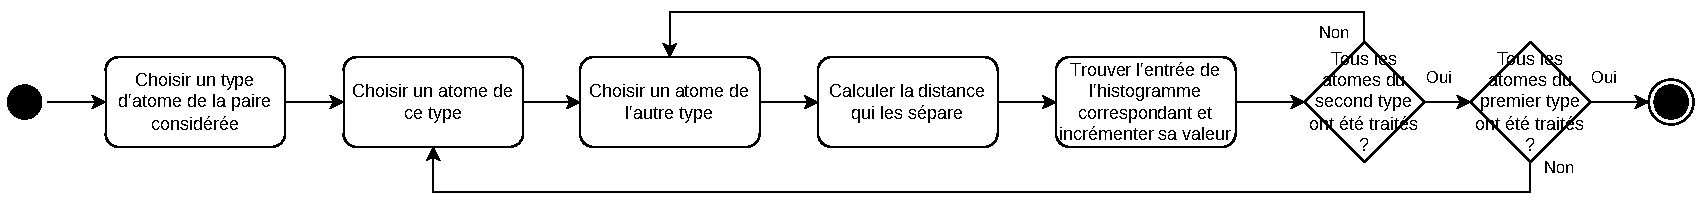
\includegraphics[width=\linewidth]{demarche-histogramme.pdf}
	\caption{Incrément de l'histogramme}
	\label{fig:histogramme}
\end{figure}

	\subsection{Moyenne et normalisation de l'histogramme}

Une fois que le fichier de configurations a été complètement parcouru, l'histogramme doit être moyenné sur le nombre de configurations traitées puis normalisé selon l'\autoref{eq:rdf} pour obtenir la fonction de distribution radiale.

\section{Déplacement carré moyen}

Le déplacement carré moyen est défini par :
\begin{equation*}
	\boxed%
	{
		MSD (t) = \frac{1}{N_{atomes}} \sum_i \left| \vec{r}_i (t) - \vec{r}_i (0) \right|^2
	}
\end{equation*}

Le calcul de cette grandeur est assez direct et intuitif, il faut simplement veiller à comparer les positions des mêmes atomes, car dans le fichier de sortie de LAMMPS, les atomes ne sont pas forcément dans le même ordre d'une configuration à une autre.

\section{Résultats obtenus}

Pour tester l'implémentation, une simulation LAMMPS est effectuée.

Le système est de l'eau à l'état liquide à \qty{300}{\kelvin} avec une densité de \num{1}. La boîte de simulation est cubique de côté \qty{20}{\angstrom}.\\
En suivant la démarche précédente (sur la préparation de système pour LAMMPS), le nombre de molécules d'eau est fixé à \num{267}, et celles-ci sont placées dans la boîte avec PACKMOL.\\
Pour s'assurer que le système est stable, son énergie et ses forces sont minimisés avec LAMMPS. Ceci fait, la simulation de dynamique moléculaire est lancée avec un pas de temps de \qty{.5}{\femto\second} pour \num{50000} pas, soit une durée de \qty{25}{\pico\second}.

Lorsque la simulation est terminée, nous obtenons les trajectoires des atomes et quelques quantités thermodynamiques.

\begin{figure}[hbpt]
	\centering
	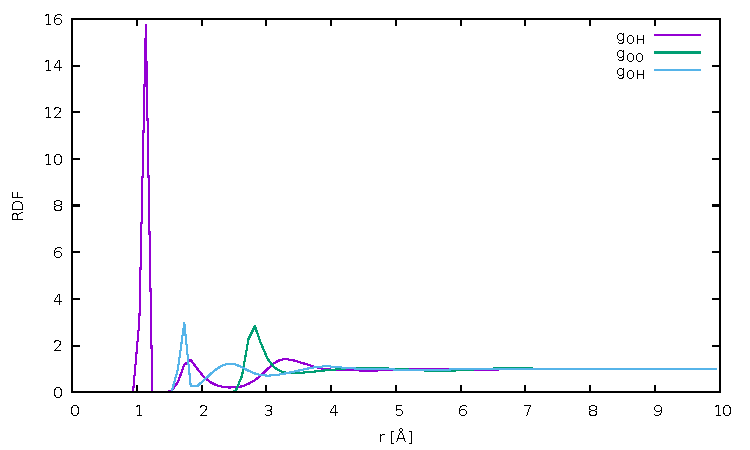
\includegraphics[width=\linewidth]{RDF.pdf}
	\caption{Fonction de distribution radiale obtenue}
	\label{fig:rdf_obtenue}
\end{figure}

La \autoref{fig:rdf_obtenue} montre des résultats qui semblent cohérents avec le système, c'est-à-dire :
\begin{itemize}
	\item des pics aux alentours de \num{.96} et \qty{1.97}{\angstrom} pour $g_{OH}$
	\item un pic aux alentours de \qty{1.8}{\angstrom} pour $g_{HH}$
	\item un pic autour de \qty{2.8}{\angstrom} pour $g_{OO}$
\end{itemize}

\begin{figure}[hptb]
	\centering
	\begin{subfigure}{\linewidth}
		\centering
		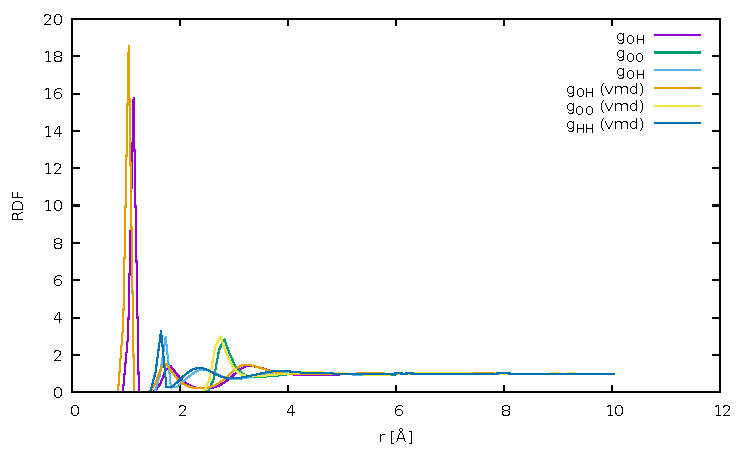
\includegraphics[width=\linewidth]{RDF-comp.pdf}
		\caption{Comparaison brute}
		\label{fig:rdf_comp_brute}
	\end{subfigure}
	
	\begin{subfigure}{\linewidth}
		\centering
		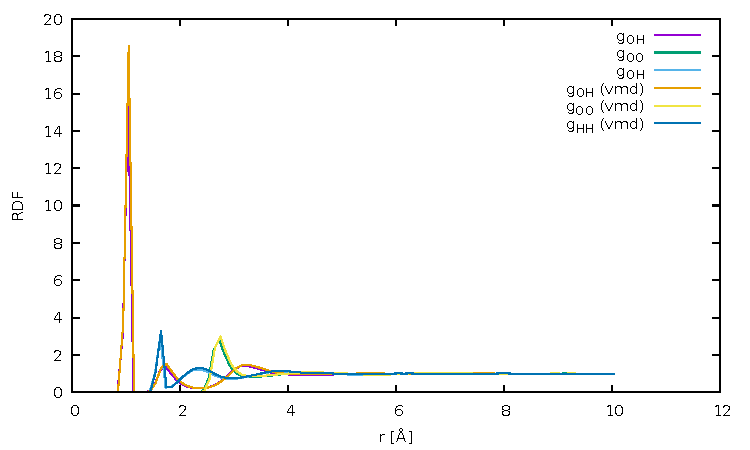
\includegraphics[width=\linewidth]{RDF-comp-shifted.pdf}
		\caption{Comparaison avec décalage}
		\label{fig:rdf_comp_decalee}
	\end{subfigure}
	\caption{Comparaison des résultats avec VMD}
	\label{fig:rdf_comp}
\end{figure}

La \autoref{fig:rdf_comp_brute} montre que les résultats ne sont pas exactement identiques à ceux obtenus avec VMD : les trois courbes sont légèrement décalées suivant les abscisses.\\
La \autoref{fig:rdf_comp_decalee} est obtenue en décalant les abscisses des courbes de $\delta r$ vers les négatifs : nous pouvons voir que les pics sont localisés aux mêmes abscisses mais que leurs amplitudes diffèrent légèrement.

Il est possible que le problème d'amplitude soit lié au problème d'abscisses : le problème des abscisses est dû à des nombres de paliers différents entre le calcul de VMD et le calcul implémenté, or la normalisation de l'histogramme (\autoref{eq:rdf}) nécessite de calculer le volume des coquilles correspondant à chaque palier. Nous pouvons alors supposer que si les paliers sont décalés, les volumes le sont également et les valeurs de la RDF sont différentes.

La \autoref{fig:msd} montre les résultats obtenus pour le déplacement carré moyen. Ces résultats sont identiques à ceux de VMD (\autoref{fig:rmsd_comp}).

\begin{figure}[hpbt]
	\centering
	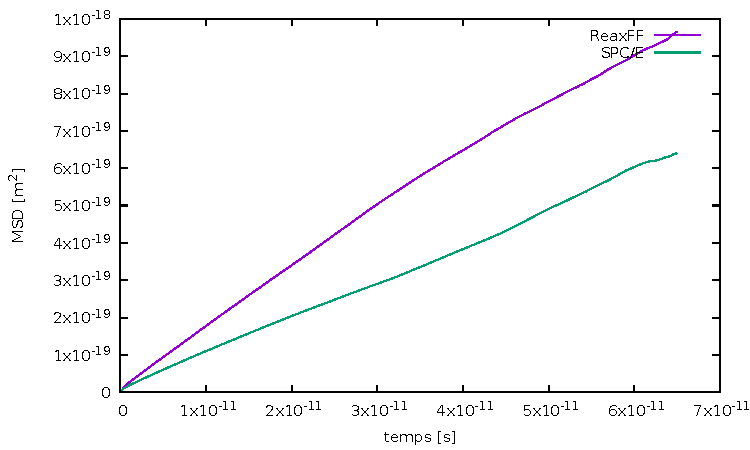
\includegraphics[width=\linewidth]{MSD.pdf}
	\caption{Déplacement carré moyen obtenu}
	\label{fig:msd}
\end{figure}

\begin{figure}[hptb]
	\centering
	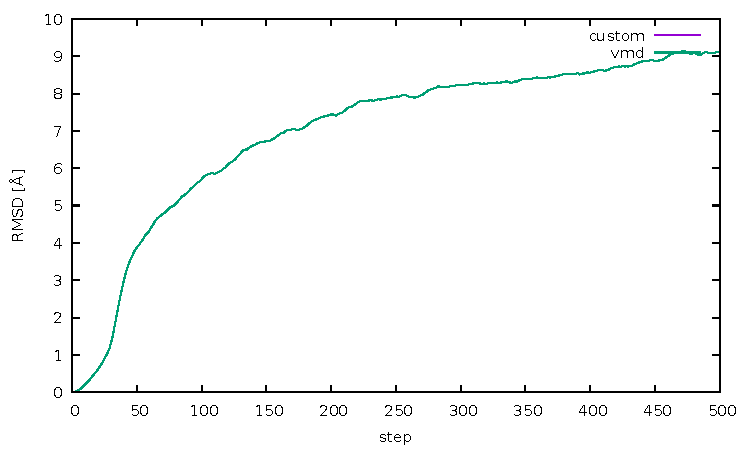
\includegraphics[width=\linewidth]{RMSD-comp.pdf}
	\caption{Comparaison avec VMD}
	\label{fig:rmsd_comp}
\end{figure}

\end{document}